% =====================================================================
%  resultados_6.tex  --  Sección de Resultados (se incluye desde main_6.tex)
% ---------------------------------------------------------------------
%  Borrador iniciado el 5-nov-2026 a partir de results_finales/ANALISIS_RESULTADOS_DISCUSION.md.
%  - Tablas: \input de los .tex generados por r2_tablas.m, r4_inferencia.m y
%    r8_tiempos_adversarial.m (no editar a mano; se regeneran con esos scripts).
%  - Figuras: PDF de results_finales/figuras/ y results_finales/complementarias/ (requiere graphicx).
%  - Cada cifra del texto se copió de un CSV; la fuente va en el comentario %%% [fuente] del párrafo.
%  - Resultados de prueba: descriptivos salvo los intervalos del bootstrap. La interpretación
%    (mecanismos, comparación con la literatura) se deja para la Discusión.
% =====================================================================

\section{Resultados}\label{sec:resultados}

Esta sección presenta los resultados en el orden del protocolo: primero la estabilidad numérica de la implementación, después la validación y la selección de parámetros (2015--2018) y, por último, la evaluación fuera de muestra (2019--2025). Se usa la notación de la Tabla~\ref{tab:contrastes}: $c_1=(0.90,\,0.01)$ es la configuración elegida para la geometría~1, $c_2=(0.80,\,0.01)$ la elegida para la geometría~2, $G_g(c)$ la geometría $g$ con la configuración $c$ y $\mathrm{Nom}(\delta)$ el Kelly nominal con ese $\delta$. Las cifras del periodo de prueba son descriptivas: corresponden a una sola trayectoria por estrategia, y solo los intervalos del bootstrap (Sección~\ref{sec:res_principal}) cuantifican la incertidumbre de las diferencias.

% ---------------------------------------------------------------------
\subsection{Estabilidad numérica y verificación}\label{sec:res_estabilidad}

%%% [fuente] metricas_por_tramo.csv (meses_sin_optimizacion); tabla_maestra_validacion_G*.csv (fraccion_factible);
%%% results_estado_solver/tabla_meses_sin_optimizacion.csv; results_verificaciones/*.csv; results_pruebas_21_4/pruebas_21_4.csv;
%%% results_bootstrap/test_simulado.csv; complementarias/tabla_g_tiempos.csv.
Ningún mes quedó sin optimizar. En las seis estrategias evaluadas y en los dos tramos todos los problemas mensuales terminaron con solución óptima, y lo mismo ocurrió en todas las celdas de la malla: la fracción de meses con solución óptima es igual a 1 en las 66 combinaciones $(\delta,\eta)$ de cada geometría durante la validación y en los 132 meses de la malla completa de la geometría~1, sin estados inexactos, certificados de infactibilidad ni fallos numéricos. Esto concuerda con el hecho, señalado en la Sección~\ref{sec:protocolo}, de que con $\delta\le 0.90$ el problema siempre es factible.

Las verificaciones de la Sección~\ref{sec:impl} se cumplieron todas. (a) Con $\eta=0$, el modelo Wasserstein--Kelly reproduce exactamente al nominal en el backtest completo de 132 meses para los seis valores de $\delta$ (diferencia máxima nula en factores de crecimiento, ponderaciones y riqueza final), y en las tres instancias individuales los valores objetivo del nominal y de las dos geometrías coinciden, con solución única. (b) En las 132 celdas comprobadas, el residuo máximo del balance fue $1.9\times10^{-10}$, sin incumplimientos de los límites por activo ni de la cota de supervivencia en la ventana. (d)--(f) Las 153 comprobaciones de la instancia sintética, del problema adversarial primal y dual y de la monotonía en el radio quedaron dentro de sus tolerancias; en particular, el óptimo del solucionador difiere del máximo de la búsqueda exhaustiva en $1.1\times10^{-7}$ y los valores primal y dual del problema adversarial coinciden hasta $5.6\times10^{-9}$ en las instancias reales.

La Tabla~\ref{tab:tiempos} resume el tiempo de solución. Cada problema mensual de Wasserstein--Kelly se resolvió en una mediana de $0.122$--$0.124$~s en prueba, frente a $0.090$~s del nominal, con un máximo de $0.323$~s; en prueba, la construcción de la matriz de costos y del radio tomó entre $0.45$ y $0.58$~ms por mes. Por último, el procedimiento de bootstrap se comprobó con series simuladas AR(1): la media se estimó sin sesgo apreciable ($0.0020001$ frente a $0.002$), pero la cobertura empírica del intervalo del $95\,\%$ fue $0.90$ con $\ell=3$ y $\ell=6$ y $0.864$ con $\ell=12$. Los intervalos reportados más adelante son, por tanto, algo más estrechos de lo nominal.

% Generado por results_finales/r8_tiempos_adversarial.m; no editar a mano.
\begin{table}[h]
\centering
\footnotesize
\setlength{\tabcolsep}{4pt}
\caption{Tiempo de solución por mes (segundos) de cada problema mensual, re-resuelto con el portafolio heredado guardado (modelado en CVX y solución con MOSEK). $C_k$ y $\rho_k$: construcción de la matriz de costos y del radio (milisegundos, prueba). Una medición por mes; MATLAB R2026a, CVX Version 2.2, Build 1148, MOSEK 9.1.9, 8 núcleos.}\label{tab:tiempos}
\begin{tabular}{|l|r|r|r|r|r|r|r|}
\hline
 & \multicolumn{3}{c|}{\textbf{Prueba (84)}} & \multicolumn{2}{c|}{\textbf{Validación (48)}} & & \\ \cline{2-6}
\textbf{Estrategia} & \textbf{Mediana} & \textbf{Media} & \textbf{Máx.} & \textbf{Mediana} & \textbf{Máx.} & \textbf{$C_k$, $\rho_k$ (ms)} & \textbf{No óptimos} \\ \hline
Nominal (0.80) & 0.090 & 0.091 & 0.099 & 0.091 & 0.231 & 0.00 & 0 \\ \hline
Nominal (0.90) & 0.090 & 0.091 & 0.103 & 0.090 & 0.096 & 0.00 & 0 \\ \hline
G1 (0.80, 0.01) & 0.124 & 0.124 & 0.135 & 0.123 & 0.150 & 0.45 & 0 \\ \hline
G1 (0.90, 0.01) & 0.122 & 0.124 & 0.144 & 0.123 & 0.133 & 0.45 & 0 \\ \hline
G2 (0.80, 0.01) & 0.124 & 0.125 & 0.142 & 0.124 & 0.136 & 0.58 & 0 \\ \hline
G2 (0.90, 0.01) & 0.123 & 0.128 & 0.323 & 0.123 & 0.132 & 0.57 & 0 \\ \hline
\end{tabular}
\end{table}


% ---------------------------------------------------------------------
\FloatBarrier %%% [R-res] las flotantes de la subsección anterior no pasan de aquí
\subsection{Validación y selección de parámetros}\label{sec:res_validacion}

%%% [fuente] results_seleccion/riqueza_vs_eta.csv (perdida_rel_vs_eta0); RESULTADOS.md §2.10; tabla_f_validacion_referencias.csv;
%%% results_estado_solver/diagnostico_eta_alto.csv; results_seleccion/diagnostico_cota_delta.csv.
La Figura~\ref{fig:mapa_riqueza} muestra la riqueza final de validación en la malla $\delta\times\eta$ y la Figura~\ref{fig:riqueza_eta}, su evolución con $\eta$. El patrón es el mismo en las dos geometrías: la riqueza depende poco de $\delta$ y cae con $\eta$. Con $\eta$ fijo, la diferencia relativa máxima entre valores de $\delta$ es $0.458\,\%$ en la geometría~1 y $0.081\,\%$ en la geometría~2. En cambio, todo $\eta>0$ reduce la riqueza frente a $\eta=0$: con $\eta=0.01$ la pérdida relativa es $1.52\,\%$ para la geometría~1 con $\delta=0.90$ y $1.06\,\%$ para la geometría~2 con $\delta=0.80$; con $\eta=0.10$ llega a $28.4\,\%$ y $24.2\,\%$. Con $\delta=0.90$ y $\eta$ entre $0.02$ y $0.15$, la geometría~2 pierde menos que la geometría~1 con el mismo $\eta$ (con $\eta=0.10$, riqueza de $1.793$ frente a $1.694$), salvo con $\eta=0.03$, donde quedan prácticamente iguales ($2.184$ frente a $2.186$).

Con $\eta\ge0.30$ las dos geometrías trasladan prácticamente toda la riqueza al activo de bajo riesgo: la riqueza de validación queda entre $1.0318$ y $1.0320$ para todo $\delta$, el mismo nivel del activo de bajo riesgo ($1.032$, Tabla~\ref{tab:r2_f}). La Figura~\ref{fig:exposicion_eta} ilustra este cambio para la geometría~1 con $\delta=0.90$: con $\eta=0$ y $\eta=0.10$ la proporción invertida en riesgo se mantiene cercana a 1 en casi todos los meses, con $\eta=0.15$ aparecen tramos sin exposición y con $\eta=0.30$ la exposición es prácticamente nula en casi toda la trayectoria. En validación, la cota $\delta$ solo estuvo activa en alguna celda con $\delta=0.90$, y el nominal con $\delta=0.80$ y con $\delta=0.90$ terminó con la misma riqueza ($2.367$).

%%% [fuente] results_seleccion/sensibilidad_seleccion.csv; top10_G2.csv; RESULTADOS.md §3.8.
%%% [R-res] Reúne los pasajes marcados %%% [RESULTADO] de la selección en metodologia_6.tex; decidir si se retiran de allí (P2).
Con la regla de selección de la Sección~\ref{sec:protocolo}, la geometría~1 eligió $c_1=(0.90,\,0.01)$, la celda con mayor riqueza entre las de $\eta>0$ ($2.331$), que está en el borde de la malla: el mayor $\delta$ y el menor $\eta$ positivo. Esta elección no cambia al multiplicar o dividir por diez la tolerancia de empate, y coincide con la de mayor Sharpe. La geometría~2 eligió $c_2=(0.80,\,0.01)$ ($2.342$), tercera en riqueza, por la regla de desempate: cinco celdas con $\eta=0.01$ quedaron dentro de la tolerancia $\mathrm{TOL}=5\times10^{-4}$. Esta elección sí depende de la tolerancia: con $10\,\mathrm{TOL}$ se habría elegido $(0.90,\,0.01)$ y con $\mathrm{TOL}/10$, $(0.75,\,0.01)$. Si $\eta=0$ hubiera sido elegible, ambas geometrías habrían seleccionado el nominal con $\delta=0.90$ (riqueza $2.367$). La Tabla~\ref{tab:r2_d} compara las configuraciones elegidas con el nominal en validación: este tiene la mayor riqueza, mientras que las configuraciones robustas tienen menor turnover ($4.13$ y $4.04$ frente a $4.73$ y $4.70$) y menor VaR.

\begin{figure}[htbp]
\centering
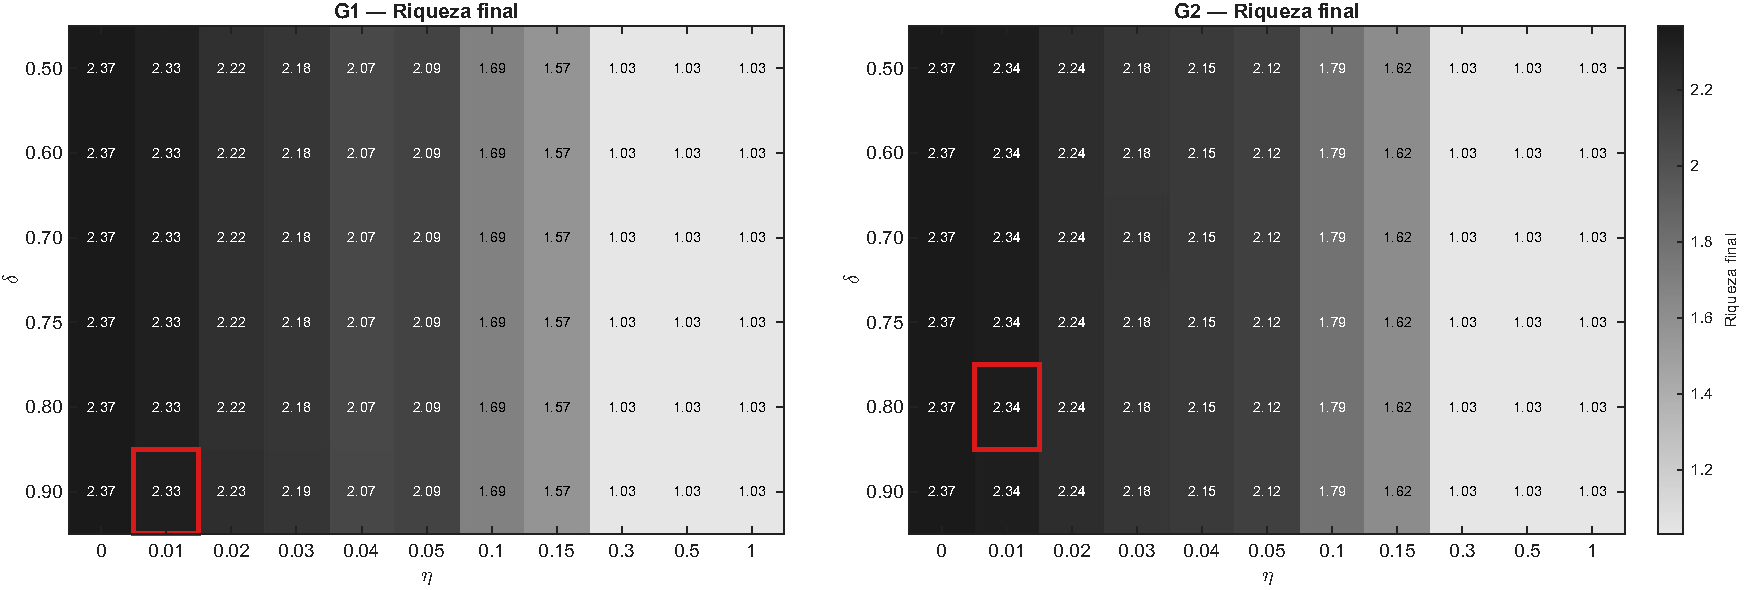
\includegraphics[width=\textwidth]{results_finales/figuras/mapa_riqueza.pdf}
\caption{Validación 2015--2018: riqueza final en la malla $\delta\times\eta$ para cada geometría. El recuadro marca la configuración elegida.}\label{fig:mapa_riqueza}
\end{figure}

\begin{figure}[htbp]
\centering
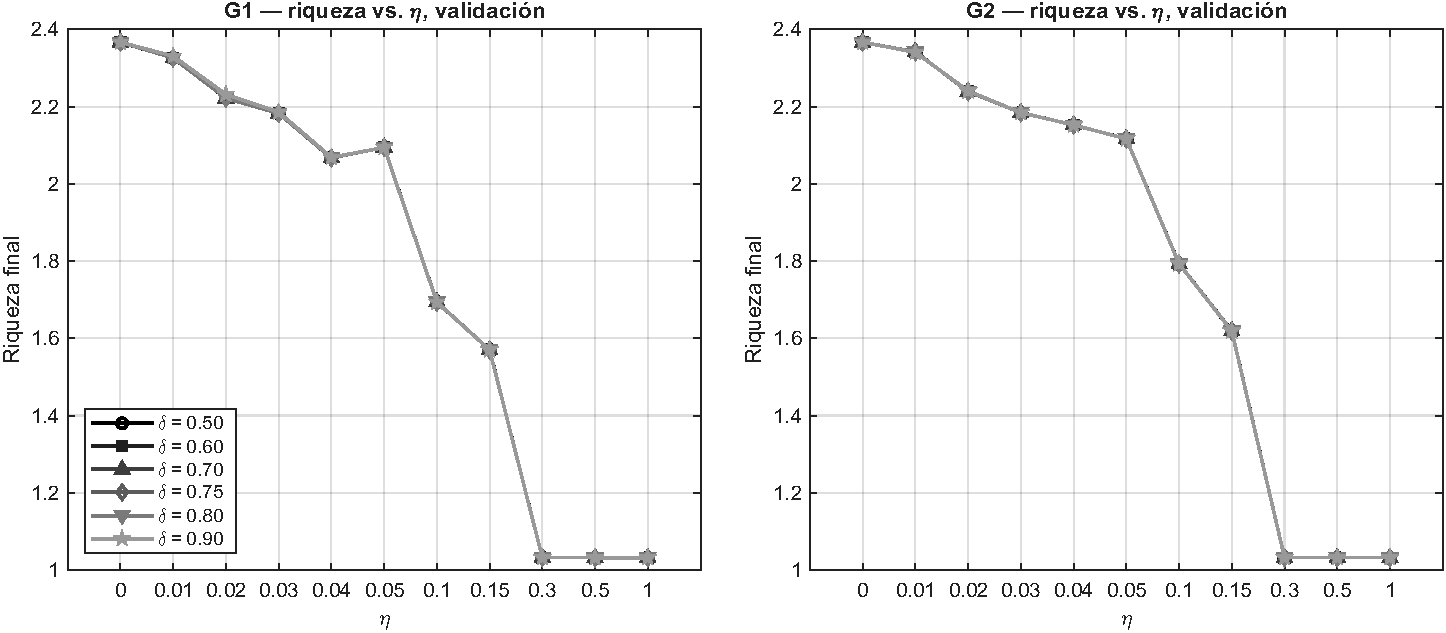
\includegraphics[width=\textwidth]{results_finales/figuras/riqueza_vs_eta_validacion.pdf}
\caption{Validación 2015--2018: riqueza final frente a $\eta$ (espaciado categórico), una línea por valor de $\delta$.}\label{fig:riqueza_eta}
\end{figure}

\begin{figure}[htbp]
\centering
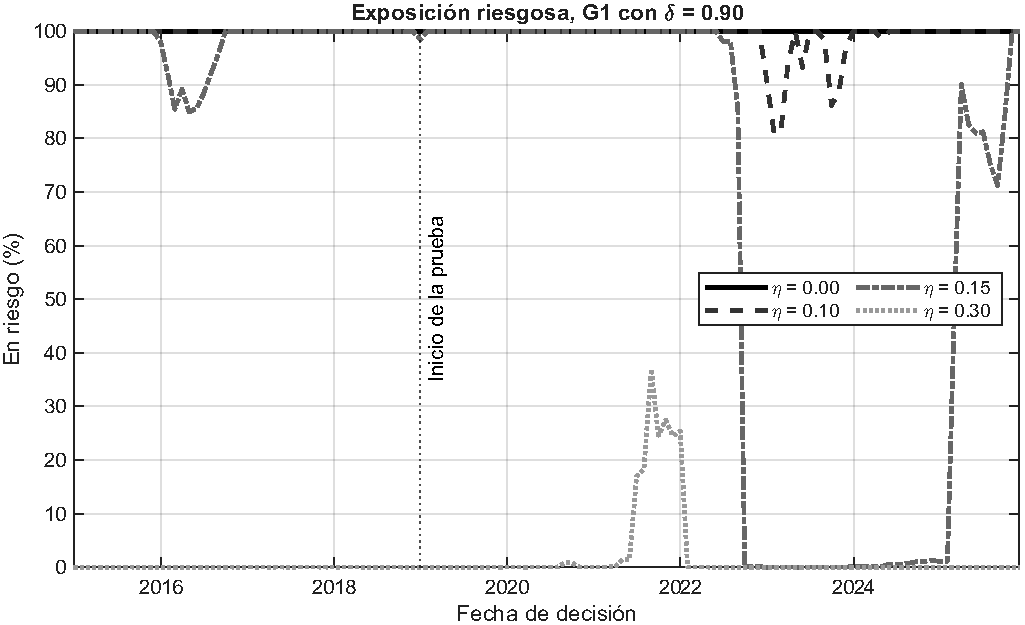
\includegraphics[width=0.85\textwidth]{results_finales/figuras/exposicion_eta_alto.pdf}
\caption{Proporción invertida en activos riesgosos de la geometría~1 con $\delta=0.90$ y $\eta\in\{0,\,0.10,\,0.15,\,0.30\}$ en las 132 fechas de decisión.}\label{fig:exposicion_eta}
\end{figure}

% Generado por results_finales/r2_tablas.m; no editar a mano.
\begin{table}[h]
\centering
\footnotesize
\setlength{\tabcolsep}{4pt}
\caption{Validación 2015--2018: configuraciones elegidas y Kelly nominal con el mismo $\delta$. $c_1=(0.90,\,0.01)$, $c_2=(0.80,\,0.01)$, $\delta_1^\star=0.90$, $\delta_2^\star=0.80$; $^{\dagger}$~configuración elegida en validación.}\label{tab:r2_d}
\begin{tabular}{|l|r|r|r|r|}
\hline
\textbf{Métrica} & \textbf{$\mathrm{Nom}(\delta_2^\star)$} & \textbf{$\mathrm{Nom}(\delta_1^\star)$} & \textbf{$G_1(c_1)^{\dagger}$} & \textbf{$G_2(c_2)^{\dagger}$} \\ \hline
Riqueza final ($W_0=1$) & 2.367 & 2.367 & 2.331 & 2.342 \\ \hline
Crecimiento logarítmico medio mensual & 1.79\,\% & 1.79\,\% & 1.76\,\% & 1.77\,\% \\ \hline
CAGR & 24.03\,\% & 24.03\,\% & 23.56\,\% & 23.70\,\% \\ \hline
Máxima caída (MDD) & 19.59\,\% & 19.59\,\% & 19.59\,\% & 19.74\,\% \\ \hline
Peor mes & $-$10.86\,\% & $-$10.86\,\% & $-$10.86\,\% & $-$10.86\,\% \\ \hline
VaR 95\,\% (pérdida mensual) & 6.53\,\% & 6.53\,\% & 5.98\,\% & 6.25\,\% \\ \hline
CVaR 95\,\% (pérdida mensual) & 9.01\,\% & 9.01\,\% & 8.92\,\% & 9.12\,\% \\ \hline
Sharpe & 1.311 & 1.311 & 1.306 & 1.313 \\ \hline
Sortino & 2.608 & 2.608 & 2.612 & 2.584 \\ \hline
Calmar & 1.227 & 1.227 & 1.203 & 1.201 \\ \hline
Turnover acumulado & 4.73 & 4.70 & 4.13 & 4.04 \\ \hline
Meses con transacción & 48 & 48 & 48 & 48 \\ \hline
Costo fraccional acumulado & 0.47\,\% & 0.47\,\% & 0.41\,\% & 0.40\,\% \\ \hline
Costo monetario acumulado ($W_0=1$) & 0.0068 & 0.0067 & 0.0060 & 0.0057 \\ \hline
Peso máximo medio & 25.00\,\% & 25.00\,\% & 25.00\,\% & 25.00\,\% \\ \hline
$N_{\mathrm{eff}}$ medio & 4.22 & 4.23 & 4.34 & 4.33 \\ \hline
Proporción en riesgo media & 99.99\,\% & 99.99\,\% & 99.99\,\% & 99.99\,\% \\ \hline
\end{tabular}
\end{table}


% ---------------------------------------------------------------------
\FloatBarrier %%% [R-res] las flotantes de la subsección anterior no pasan de aquí
\subsection{Desempeño fuera de muestra}\label{sec:res_prueba}

%%% [fuente] tabla_a_prueba_desempeno.csv; contrastes_prueba.csv (riqueza_A_sobre_B_menos_1).
Las Tablas~\ref{tab:r2_a} a \ref{tab:r2_c} reúnen las métricas de las seis estrategias en el periodo de prueba, y la Figura~\ref{fig:riqueza_prueba} muestra sus trayectorias de riqueza. Las cuatro estrategias Wasserstein--Kelly terminaron con más riqueza que el nominal con el mismo $\delta$: $G_1(c_1)$ alcanzó $3.999$ frente a $3.741$ de $\mathrm{Nom}(0.90)$ ($6.9\,\%$ más), $G_2(c_2)$ $3.873$ frente a $3.625$ de $\mathrm{Nom}(0.80)$ ($6.8\,\%$ más), $G_2(c_1)$ $3.873$ ($3.5\,\%$ más que $\mathrm{Nom}(0.90)$) y $G_1(c_2)$ $3.686$ ($1.7\,\%$ más que $\mathrm{Nom}(0.80)$). En validación el orden había sido el contrario (Tabla~\ref{tab:r2_d}). Las tasas de crecimiento anual compuesto van de $20.20\,\%$ a $21.90\,\%$ y el crecimiento logarítmico medio mensual, de $1.53\,\%$ a $1.65\,\%$. Con $\delta=0.90$, la geometría~1 terminó con más riqueza que la geometría~2 ($3.999$ frente a $3.873$); con $\delta=0.80$ ocurrió lo contrario ($3.686$ frente a $3.873$).

%%% [fuente] tabla_a_prueba_desempeno.csv; tabla_c_prueba_restricciones.csv; r2_cota_delta.csv.
Las diferencias en pérdidas son pequeñas (Figura~\ref{fig:drawdown_prueba}). La máxima caída va de $25.54\,\%$ ($G_1(c_1)$) a $27.04\,\%$ ($G_1(c_2)$), el peor mes de $-11.11\,\%$ a $-12.13\,\%$ y el CVaR al $95\,\%$ de $9.77\,\%$ a $10.55\,\%$; con 84 meses, estas medidas de cola descansan en unos cuatro meses. El Sharpe va de $0.891$ ($\mathrm{Nom}(0.80)$) a $1.002$ ($G_1(c_1)$). En cuanto a la supervivencia (Tabla~\ref{tab:r2_c}), las tres estrategias con $\delta=0.90$ tuvieron dos meses de prueba con factor de crecimiento realizado por debajo de $0.90$ (mínimos de $0.8859$, $0.8886$ y $0.8865$), mientras que las de $\delta=0.80$ no tuvieron ninguno por debajo de $0.80$. Con $\delta=0.90$, la cota estuvo activa en la ventana en 60 a 66 de los 84 meses; con $\delta=0.80$, en ninguno.

%%% [fuente] tabla_b_prueba_operacion.csv.
La Tabla~\ref{tab:r2_b} y la Figura~\ref{fig:turnover_prueba} describen la operación. Las estrategias Wasserstein--Kelly rotaron menos que el nominal con el mismo $\delta$: turnover acumulado de $7.92$ ($G_1(c_2)$) y $7.05$ ($G_2(c_2)$) frente a $8.73$ con $\delta=0.80$, y de $6.59$ ($G_1(c_1)$) y $6.77$ ($G_2(c_1)$) frente a $7.60$ con $\delta=0.90$. El costo monetario acumulado, en unidades de riqueza inicial, fue de $0.0159$ a $0.0192$ en las estrategias robustas, frente a $0.0216$ y $0.0180$ del nominal. Todas las estrategias estuvieron prácticamente invertidas por completo (proporción media en riesgo de $99.94\,\%$ a $99.99\,\%$), con el peso máximo en la cota $\bar x=0.25$ y un número efectivo de activos riesgosos de $4.25$ a $4.71$; las robustas tuvieron un $N_{\mathrm{eff}}$ algo mayor que el nominal del mismo $\delta$.

% Generado por results_finales/r2_tablas.m; no editar a mano.
\begin{table}[h]
\centering
\footnotesize
\setlength{\tabcolsep}{4pt}
\caption{Prueba 2019--2025: desempeño de las seis estrategias evaluadas. $c_1=(0.90,\,0.01)$, $c_2=(0.80,\,0.01)$, $\delta_1^\star=0.90$, $\delta_2^\star=0.80$; $^{\dagger}$~configuración elegida en validación.}\label{tab:r2_a}
\begin{tabular}{|l|r|r|r|r|r|r|}
\hline
\textbf{Métrica} & \textbf{$\mathrm{Nom}(\delta_2^\star)$} & \textbf{$\mathrm{Nom}(\delta_1^\star)$} & \textbf{$G_1(c_2)$} & \textbf{$G_1(c_1)^{\dagger}$} & \textbf{$G_2(c_2)^{\dagger}$} & \textbf{$G_2(c_1)$} \\ \hline
Riqueza final ($W_0=1$) & 3.625 & 3.741 & 3.686 & 3.999 & 3.873 & 3.873 \\ \hline
Crecimiento logarítmico medio mensual & 1.53\,\% & 1.57\,\% & 1.55\,\% & 1.65\,\% & 1.61\,\% & 1.61\,\% \\ \hline
CAGR & 20.20\,\% & 20.74\,\% & 20.48\,\% & 21.90\,\% & 21.34\,\% & 21.34\,\% \\ \hline
Máxima caída (MDD) & 26.39\,\% & 26.79\,\% & 27.04\,\% & 25.54\,\% & 26.38\,\% & 26.42\,\% \\ \hline
Peor mes & $-$12.13\,\% & $-$11.41\,\% & $-$11.11\,\% & $-$11.14\,\% & $-$11.95\,\% & $-$11.35\,\% \\ \hline
VaR 95\,\% (pérdida mensual) & 8.48\,\% & 8.35\,\% & 8.48\,\% & 8.35\,\% & 8.48\,\% & 8.26\,\% \\ \hline
CVaR 95\,\% (pérdida mensual) & 10.55\,\% & 10.04\,\% & 10.05\,\% & 9.77\,\% & 10.32\,\% & 9.80\,\% \\ \hline
Sharpe & 0.891 & 0.947 & 0.917 & 1.002 & 0.952 & 0.981 \\ \hline
Sortino & 1.779 & 1.924 & 1.841 & 2.049 & 1.904 & 2.005 \\ \hline
Calmar & 0.765 & 0.774 & 0.758 & 0.857 & 0.809 & 0.808 \\ \hline
\end{tabular}
\end{table}

% Generado por results_finales/r2_tablas.m; no editar a mano.
\begin{table}[h]
\centering
\footnotesize
\setlength{\tabcolsep}{4pt}
\caption{Prueba 2019--2025: operación y concentración. $c_1=(0.90,\,0.01)$, $c_2=(0.80,\,0.01)$, $\delta_1^\star=0.90$, $\delta_2^\star=0.80$; $^{\dagger}$~configuración elegida en validación.}\label{tab:r2_b}
\begin{tabular}{|l|r|r|r|r|r|r|}
\hline
\textbf{Métrica} & \textbf{$\mathrm{Nom}(\delta_2^\star)$} & \textbf{$\mathrm{Nom}(\delta_1^\star)$} & \textbf{$G_1(c_2)$} & \textbf{$G_1(c_1)^{\dagger}$} & \textbf{$G_2(c_2)^{\dagger}$} & \textbf{$G_2(c_1)$} \\ \hline
Turnover acumulado & 8.73 & 7.60 & 7.92 & 6.59 & 7.05 & 6.77 \\ \hline
Meses con transacción & 84 & 84 & 84 & 84 & 84 & 84 \\ \hline
Costo fraccional acumulado & 0.87\,\% & 0.76\,\% & 0.79\,\% & 0.66\,\% & 0.70\,\% & 0.68\,\% \\ \hline
Costo monetario acumulado ($W_0=1$) & 0.0216 & 0.0180 & 0.0192 & 0.0159 & 0.0181 & 0.0167 \\ \hline
Peso máximo medio & 25.00\,\% & 24.99\,\% & 25.00\,\% & 24.96\,\% & 25.00\,\% & 24.99\,\% \\ \hline
$N_{\mathrm{eff}}$ medio & 4.25 & 4.63 & 4.39 & 4.69 & 4.43 & 4.71 \\ \hline
Proporción en riesgo media & 99.99\,\% & 99.99\,\% & 99.99\,\% & 99.99\,\% & 99.99\,\% & 99.94\,\% \\ \hline
\end{tabular}
\end{table}

% Generado por results_finales/r2_tablas.m; no editar a mano.
\begin{table}[h]
\centering
\footnotesize
\setlength{\tabcolsep}{4pt}
\caption{Prueba 2019--2025: restricciones y solucionador. $c_1=(0.90,\,0.01)$, $c_2=(0.80,\,0.01)$, $\delta_1^\star=0.90$, $\delta_2^\star=0.80$; $^{\dagger}$~configuración elegida en validación.}\label{tab:r2_c}
\begin{tabular}{|l|r|r|r|r|r|r|}
\hline
\textbf{Métrica} & \textbf{$\mathrm{Nom}(\delta_2^\star)$} & \textbf{$\mathrm{Nom}(\delta_1^\star)$} & \textbf{$G_1(c_2)$} & \textbf{$G_1(c_1)^{\dagger}$} & \textbf{$G_2(c_2)^{\dagger}$} & \textbf{$G_2(c_1)$} \\ \hline
Meses con $G^{\mathrm{real}}<\delta$ & 0 & 2 & 0 & 2 & 0 & 2 \\ \hline
Mínimo factor de crecimiento realizado & 0.8787 & 0.8859 & 0.8889 & 0.8886 & 0.8805 & 0.8865 \\ \hline
Meses con la cota $\delta$ activa en la ventana & 0 & 65 & 0 & 60 & 0 & 66 \\ \hline
Meses sin optimización & 0 & 0 & 0 & 0 & 0 & 0 \\ \hline
Meses evaluados & 84 & 84 & 84 & 84 & 84 & 84 \\ \hline
\end{tabular}
\end{table}


\begin{figure}[htbp]
\centering
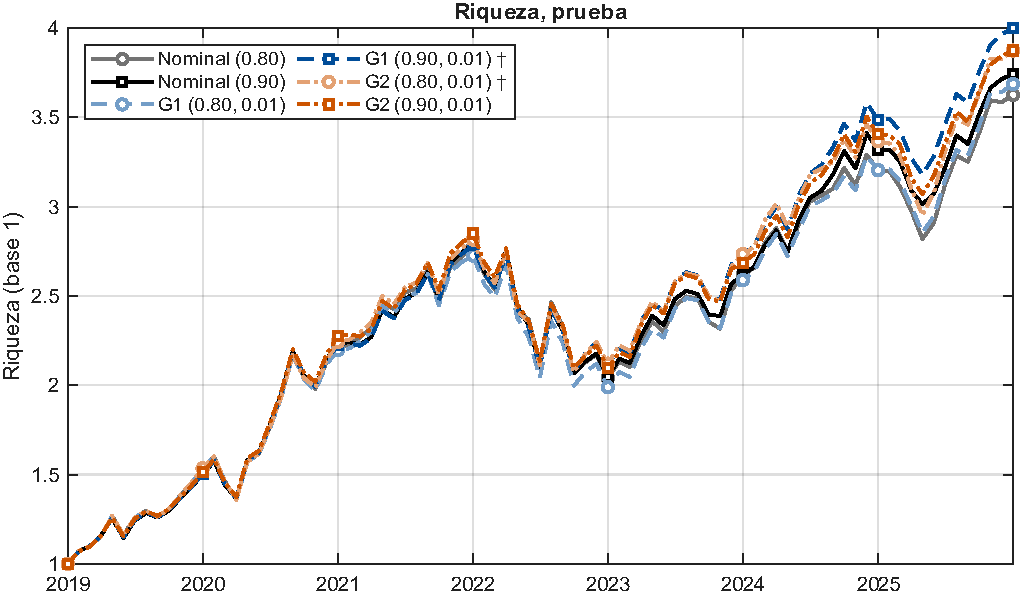
\includegraphics[width=\textwidth]{results_finales/figuras/riqueza_prueba.pdf}
\caption{Prueba 2019--2025: riqueza de las seis estrategias, re-basada a 1 al inicio del periodo.}\label{fig:riqueza_prueba}
\end{figure}

\begin{figure}[htbp]
\centering
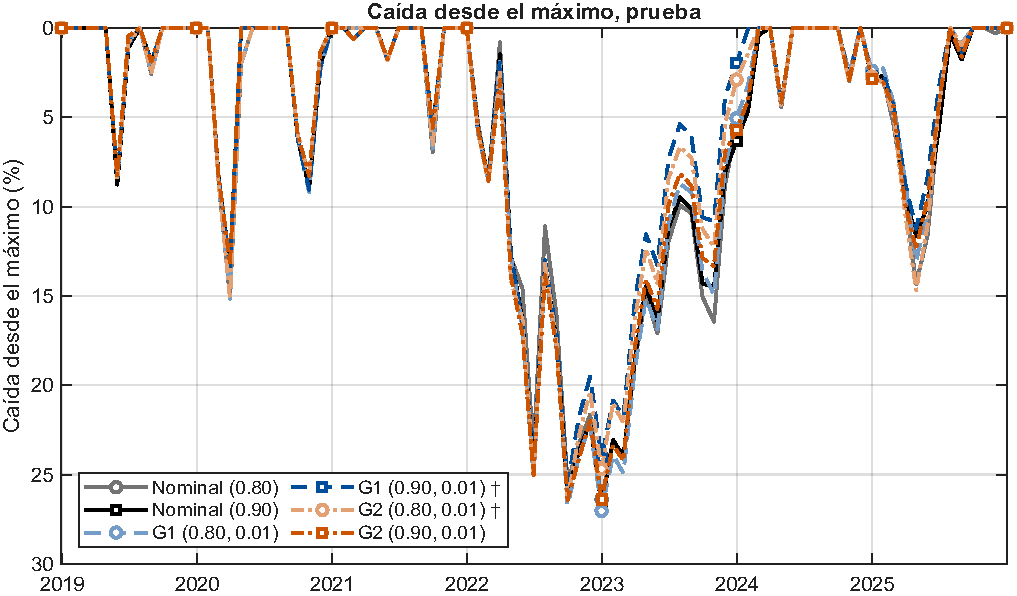
\includegraphics[width=\textwidth]{results_finales/figuras/drawdown_prueba.pdf}
\caption{Prueba 2019--2025: caída desde el máximo previo de la riqueza.}\label{fig:drawdown_prueba}
\end{figure}

\begin{figure}[htbp]
\centering
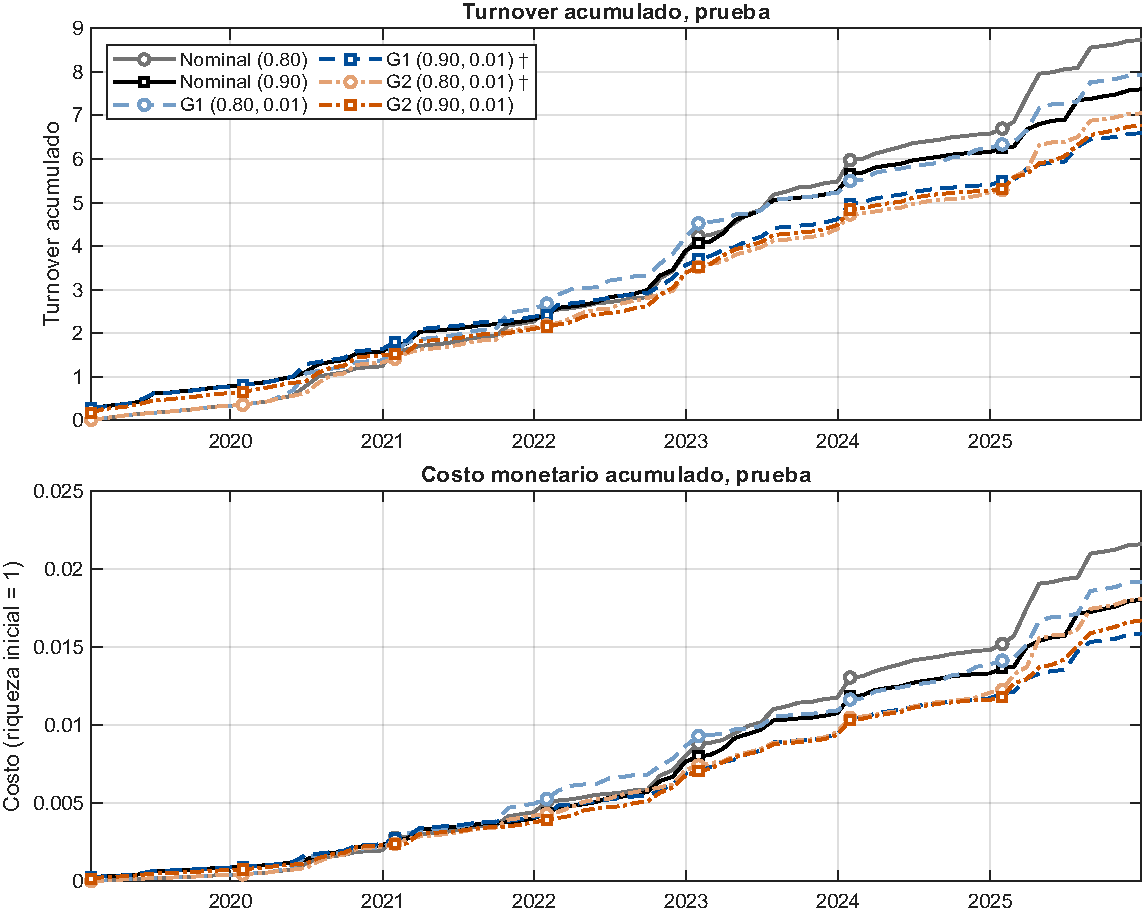
\includegraphics[width=\textwidth]{results_finales/figuras/turnover_costo_prueba.pdf}
\caption{Prueba 2019--2025: turnover acumulado y costo monetario acumulado en unidades de riqueza inicial.}\label{fig:turnover_prueba}
\end{figure}

% ---------------------------------------------------------------------
\FloatBarrier %%% [R-res] las flotantes de la subsección anterior no pasan de aquí
\subsection{Contraste principal: geometría 2 frente a geometría 1}\label{sec:res_principal}

%%% [fuente] tabla_r4a_bootstrap.csv; contrastes_prueba.csv (max_abs_D); RESULTADOS.md §2.3-2.4.
La Tabla~\ref{tab:r4_bootstrap} y la Figura~\ref{fig:ic} resumen los siete contrastes; los dos primeros forman el contraste principal, que compara las geometrías con los mismos parámetros. Con $c_1$, la media de $D_k=\log G^{G_2}_{k+1}-\log G^{G_1}_{k+1}$ es $-0.038\,\%$ mensual, con intervalo del $95\,\%$ ($\ell=6$) de $[-0.118\,\%,\ 0.038\,\%]$; con $c_2$ es $0.059\,\%$, con intervalo $[-0.035\,\%,\ 0.170\,\%]$. Ambos intervalos contienen el cero con $\ell=3$, $6$ y $12$, y las medias tienen signos opuestos. La mediana de $D_k$ es cero en los dos casos, la proporción de meses con $D_k>0$ es de $50.0\,\%$ y $52.4\,\%$, y hay 6 y 16 meses con $|D_k|<10^{-6}$. La Figura~\ref{fig:dk} muestra que las diferencias se concentran en pocos meses: la mayor diferencia mensual en valor absoluto es de $1.9$ y $2.1$ puntos porcentuales. Con los datos disponibles no hay evidencia suficiente de una diferencia media de crecimiento logarítmico entre las dos geometrías con parámetros emparejados; esto no equivale a demostrar que sean equivalentes.

% Generado por results_finales/r4_inferencia.m; no editar a mano.
\begin{table}[h]
\centering
\footnotesize
\setlength{\tabcolsep}{4pt}
\caption{Prueba 2019--2025: media de $D_k$ y su intervalo del 95\,\% por bootstrap móvil por bloques ($B=10\,000$) con $\ell\in\{3,6,12\}$. $D_k$ en \% mensual; «\% $D_k>0$» sobre los 84 meses; empates: meses con $|D_k|<10^{-6}$. Contrastes principales: 1 y 2; 3 a 7 son exploratorios y no se ajustan por comparaciones múltiples.}\label{tab:r4_bootstrap}
\begin{tabular}{|c|l|r|r|r|r|c|c|c|}
\hline
\textbf{N.º} & \textbf{Contraste} & \textbf{Media} & \textbf{Mediana} & \textbf{\% $D_k>0$} & \textbf{Empates} & \textbf{IC $\ell=3$} & \textbf{IC $\ell=6$} & \textbf{IC $\ell=12$} \\ \hline
1 & $G_2(c_1)-G_1(c_1)$ & $-$0.038 & 0.000 & 50.0 & 6 & [$-$0.118, 0.038] & [$-$0.118, 0.038] & [$-$0.126, 0.038] \\ \hline
2 & $G_2(c_2)-G_1(c_2)$ & 0.059 & 0.000 & 52.4 & 16 & [$-$0.039, 0.164] & [$-$0.035, 0.170] & [$-$0.029, 0.157] \\ \hline \hline
3 & $G_2(c_2)-G_1(c_1)$ & $-$0.038 & $-$0.061 & 42.9 & 0 & [$-$0.202, 0.133] & [$-$0.205, 0.127] & [$-$0.210, 0.076] \\ \hline
4 & $G_1(c_1)-\mathrm{Nom}(\delta_1^\star)$ & 0.079 & 0.000 & 52.4 & 7 & [0.013, 0.163] & [0.014, 0.169] & [0.007, 0.174] \\ \hline
5 & $G_2(c_1)-\mathrm{Nom}(\delta_1^\star)$ & 0.041 & 0.000 & 52.4 & 8 & [$-$0.026, 0.120] & [$-$0.021, 0.110] & [$-$0.018, 0.094] \\ \hline
6 & $G_1(c_2)-\mathrm{Nom}(\delta_2^\star)$ & 0.020 & 0.000 & 59.5 & 19 & [$-$0.079, 0.111] & [$-$0.081, 0.111] & [$-$0.084, 0.117] \\ \hline
7 & $G_2(c_2)-\mathrm{Nom}(\delta_2^\star)$ & 0.079 & 0.000 & 66.7 & 18 & [$-$0.028, 0.200] & [$-$0.035, 0.209] & [$-$0.021, 0.203] \\ \hline
\end{tabular}
\end{table}


\begin{figure}[htbp]
\centering
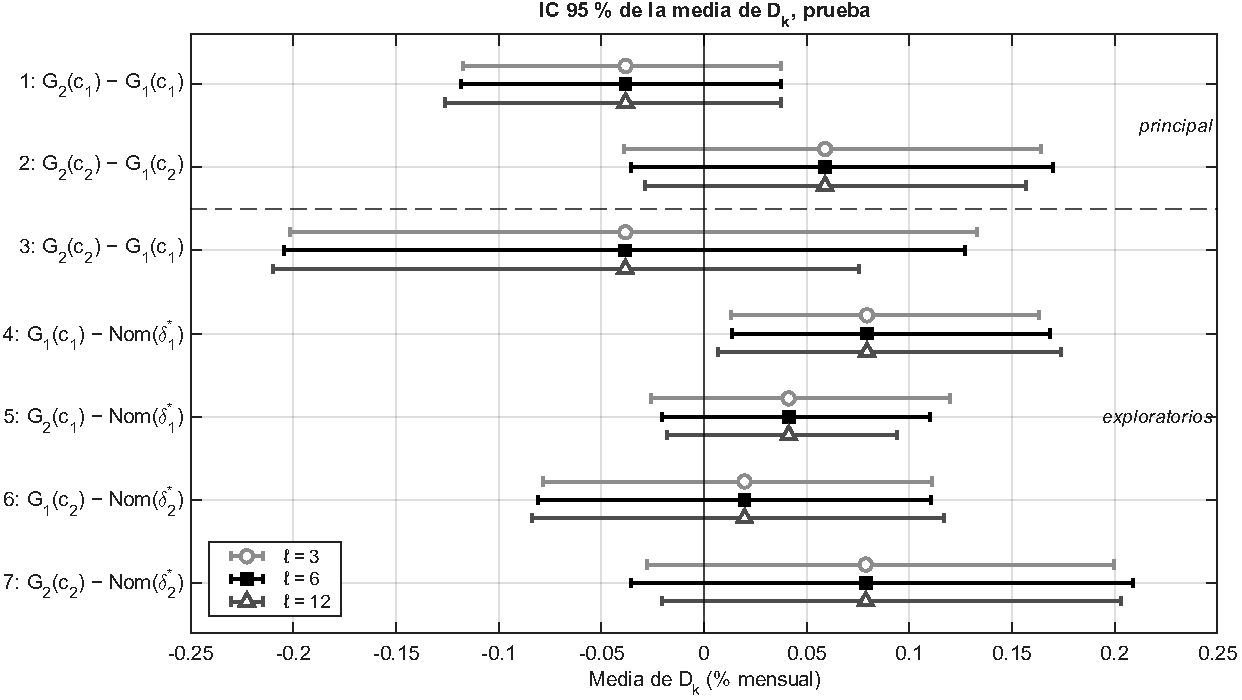
\includegraphics[width=\textwidth]{results_finales/inferencia/ic_contrastes.pdf}
\caption{Prueba 2019--2025: media de $D_k$ e intervalo del $95\,\%$ por bootstrap móvil por bloques de los siete contrastes, para $\ell\in\{3,6,12\}$. La línea discontinua separa el contraste principal de los exploratorios.}\label{fig:ic}
\end{figure}

\begin{figure}[htbp]
\centering
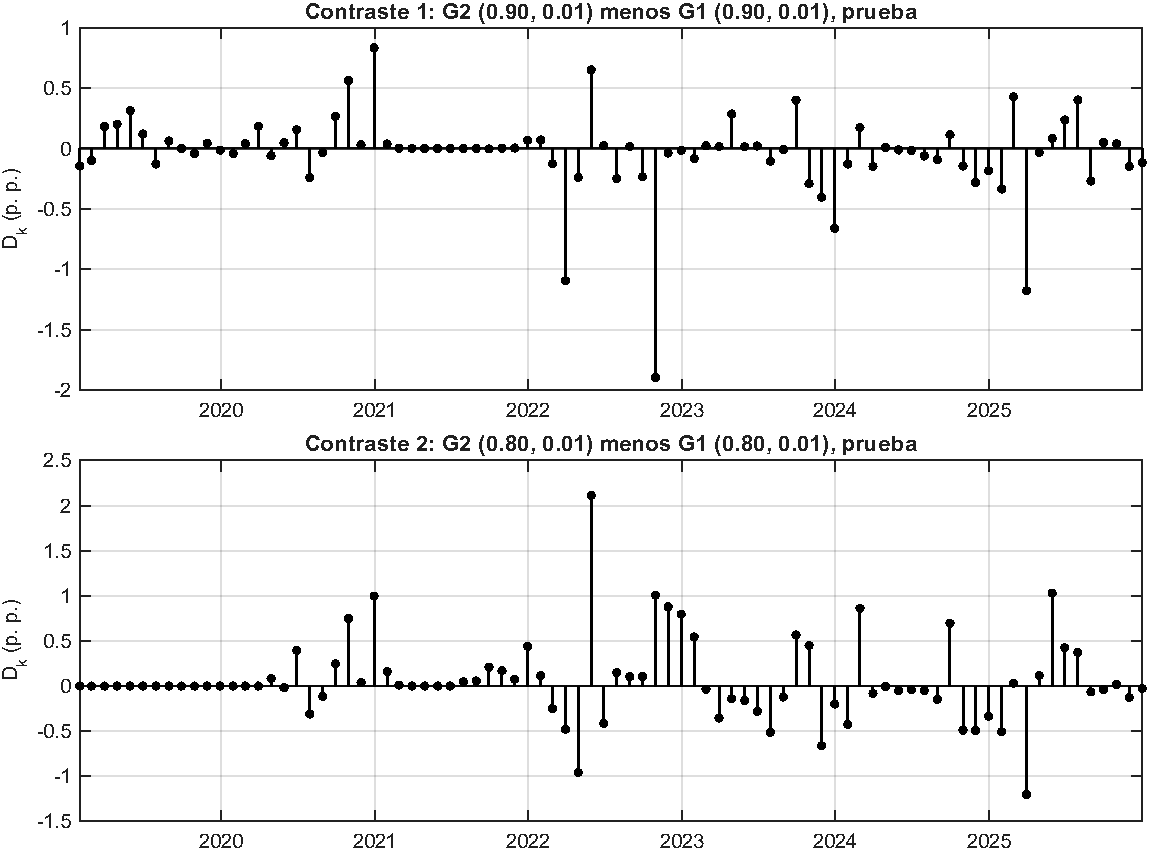
\includegraphics[width=\textwidth]{results_finales/figuras/dk_contraste_principal.pdf}
\caption{Prueba 2019--2025: diferencia mensual de crecimiento logarítmico $D_k$ (puntos porcentuales) entre las geometrías~2 y 1 con los mismos parámetros.}\label{fig:dk}
\end{figure}

% ---------------------------------------------------------------------
\FloatBarrier %%% [R-res] las flotantes de la subsección anterior no pasan de aquí
\subsection{Contrastes exploratorios y desglose por régimen}\label{sec:res_exploratorios}

%%% [fuente] tabla_r4a_bootstrap.csv; contrastes_prueba.csv.
De los contrastes exploratorios (3 a 7 de la Tabla~\ref{tab:r4_bootstrap}), solo el 4, $G_1(c_1)-\mathrm{Nom}(0.90)$, tiene un intervalo que excluye el cero con las tres longitudes de bloque: media de $0.079\,\%$ mensual e intervalo de $[0.014\,\%,\ 0.169\,\%]$ con $\ell=6$. Los otros tres contrastes frente al nominal también tienen media positiva ($0.041\,\%$, $0.020\,\%$ y $0.079\,\%$), pero sus intervalos contienen el cero. El contraste 3, entre las configuraciones elegidas para cada geometría ($G_2(c_2)-G_1(c_1)$), tiene media de $-0.038\,\%$ e intervalo $[-0.205\,\%,\ 0.127\,\%]$; como cambian a la vez la geometría y $\delta$, no se usa para identificar el efecto de la geometría. Con siete intervalos sin ajuste por multiplicidad y una cobertura empírica del bootstrap inferior a la nominal (Sección~\ref{sec:res_estabilidad}), el intervalo del contraste 4 no se interpreta como evidencia de superioridad.

%%% [fuente] tabla_r4b_regimen.csv; tabla_r4c_cruce.csv.
Las Tablas~\ref{tab:r4_regimen} y \ref{tab:r4_cruce} desglosan $D_k$ según el estado del mercado en la fecha de decisión (48 meses con VIX alto y 36 con VIX bajo; 28 con retorno de SPY negativo y 56 no negativo). En el contraste principal con $c_2$, la media es positiva con VIX alto ($0.125\,\%$, con $D_k>0$ en el $66.7\,\%$ de los meses) y con retorno de SPY negativo ($0.128\,\%$), y negativa con VIX bajo ($-0.029\,\%$). Con $c_1$ el patrón no se repite: la media es negativa con VIX alto ($-0.058\,\%$) y, sobre todo, con retorno de SPY negativo ($-0.152\,\%$). En el cruce de ambos criterios el grupo más pequeño tiene 5 meses. Este desglose es descriptivo y no incluye intervalos por grupo.

% Generado por results_finales/r4_inferencia.m; no editar a mano.
\begin{table}[h]
\centering
\footnotesize
\setlength{\tabcolsep}{4pt}
\caption{Prueba 2019--2025: desglose descriptivo por régimen. Cada celda: media de $D_k$ en \% mensual y, entre paréntesis, \% de meses del grupo con $D_k>0$. VIX alto: VIX$_k$ por encima de la mediana de su ventana; $r^{\mathrm{SPY}}_k$: retorno de SPY del mes $k$. Sin inferencia por grupo.}\label{tab:r4_regimen}
\begin{tabular}{|c|l|r|r|r|r|r|}
\hline
\textbf{N.º} & \textbf{Contraste} & \textbf{Todos} ($n=84$) & \textbf{VIX alto} ($n=48$) & \textbf{VIX bajo} ($n=36$) & \textbf{$r^{\mathrm{SPY}}_k<0$} ($n=28$) & \textbf{$r^{\mathrm{SPY}}_k\ge 0$} ($n=56$) \\ \hline
1 & $G_2(c_1)-G_1(c_1)$ & -0.038 (50.0) & -0.058 (52.1) & -0.012 (47.2) & -0.152 (46.4) & 0.019 (51.8) \\ \hline
2 & $G_2(c_2)-G_1(c_2)$ & 0.059 (52.4) & 0.125 (66.7) & -0.029 (33.3) & 0.128 (64.3) & 0.025 (46.4) \\ \hline \hline
3 & $G_2(c_2)-G_1(c_1)$ & -0.038 (42.9) & -0.095 (39.6) & 0.037 (47.2) & -0.105 (42.9) & -0.005 (42.9) \\ \hline
4 & $G_1(c_1)-\mathrm{Nom}(\delta_1^\star)$ & 0.079 (52.4) & 0.104 (45.8) & 0.047 (61.1) & 0.120 (46.4) & 0.059 (55.4) \\ \hline
5 & $G_2(c_1)-\mathrm{Nom}(\delta_1^\star)$ & 0.041 (52.4) & 0.046 (56.2) & 0.035 (47.2) & -0.033 (46.4) & 0.078 (55.4) \\ \hline
6 & $G_1(c_2)-\mathrm{Nom}(\delta_2^\star)$ & 0.020 (59.5) & -0.027 (50.0) & 0.082 (72.2) & -0.073 (46.4) & 0.066 (66.1) \\ \hline
7 & $G_2(c_2)-\mathrm{Nom}(\delta_2^\star)$ & 0.079 (66.7) & 0.098 (66.7) & 0.053 (66.7) & 0.055 (60.7) & 0.091 (69.6) \\ \hline
\end{tabular}
\end{table}

% Generado por results_finales/r4_inferencia.m; no editar a mano.
\begin{table}[h]
\centering
\footnotesize
\setlength{\tabcolsep}{4pt}
\caption{Prueba 2019--2025: cruce de VIX y retorno de SPY para los contrastes principales. Cada celda: media de $D_k$ en \% mensual, \% de meses con $D_k>0$ entre paréntesis y tamaño del grupo entre corchetes. Descriptivo.}\label{tab:r4_cruce}
\begin{tabular}{|c|l|l|r|r|}
\hline
\textbf{N.º} & \textbf{Contraste} & & \textbf{$r^{\mathrm{SPY}}_k<0$} & \textbf{$r^{\mathrm{SPY}}_k\ge 0$} \\ \hline
1 & $G_2(c_1)-G_1(c_1)$ & VIX alto & $-$0.158 (52.2) [23] & 0.034 (52.0) [25] \\ \cline{3-5}
 & & VIX bajo & $-$0.128 (20.0) [5] & 0.007 (51.6) [31] \\ \hline
2 & $G_2(c_2)-G_1(c_2)$ & VIX alto & 0.165 (69.6) [23] & 0.089 (64.0) [25] \\ \cline{3-5}
 & & VIX bajo & $-$0.041 (40.0) [5] & $-$0.027 (32.3) [31] \\ \hline
\end{tabular}
\end{table}


% ---------------------------------------------------------------------
\FloatBarrier %%% [R-res] las flotantes de la subsección anterior no pasan de aquí
\subsection{Costos de transacción y estrategias de referencia}\label{sec:res_referencias}

%%% [fuente] tabla_b_prueba_operacion.csv; tabla_e_prueba_referencias.csv; tabla_f_validacion_referencias.csv.
%%% [R-res] Las referencias se implementaron después de evaluar la prueba (sec:referencias): solo cifras descriptivas.
El Kelly nominal sin costos permite separar el efecto de los costos del de la robustez (Tabla~\ref{tab:r2_e} y Figura~\ref{fig:turnover_costos}). Sin costos, el turnover acumulado de prueba del nominal fue de $15.30$ con $\delta=0.80$ y $14.99$ con $\delta=0.90$; con $\tau=0.001$ bajó a $8.73$ y $7.60$, y con $\eta=0.01$ las estrategias robustas lo redujeron a valores de $6.59$ a $7.92$. La riqueza final del nominal sin costos fue de $3.743$ y $3.755$, por debajo de la de $G_1(c_1)$ ($3.999$) y de $G_2(c_2)$ ($3.873$), que sí pagan costos.

Entre las referencias externas (Figura~\ref{fig:riqueza_referencias}), el activo de bajo riesgo terminó la prueba con $1.206$, SPY pasivo con $3.034$ (máxima caída de $23.93\,\%$) y el portafolio de igual ponderación con $3.734$, con una máxima caída de $15.91\,\%$, un Sharpe de $1.162$ y un Calmar de $1.302$, mayores que los de todas las estrategias Kelly. En validación (Tabla~\ref{tab:r2_f}) el orden fue distinto: la igual ponderación terminó con $1.682$ y SPY pasivo con $1.316$, frente a $2.331$--$2.367$ de las estrategias Kelly de la Tabla~\ref{tab:r2_d}. No se calcularon contrastes ni intervalos frente a las referencias.

% Generado por results_finales/r2_tablas.m; no editar a mano.
\begin{table}[h]
\centering
\footnotesize
\setlength{\tabcolsep}{4pt}
\caption{Prueba 2019--2025: estrategias de referencia. $\mathrm{Nom}_{\tau=0}$: Kelly nominal sin costos ($\tau=0$), con turnover canónico $\sum_j|x_{jk}-h_{jk}|$; $\delta_1^\star=0.90$, $\delta_2^\star=0.80$. Igual ponderación: $1/d$ en cada acción, rebalanceo mensual con $\tau=0.001$. SPY pasivo: comprar y mantener, con costo solo en la compra inicial (diciembre de 2014). ---: no definido (sin exposición riesgosa o sin variación del exceso sobre $r^f$) o no aplica (SPY no pertenece al universo de diez acciones).}\label{tab:r2_e}
\begin{tabular}{|l|r|r|r|r|r|}
\hline
\textbf{Métrica} & \textbf{Bajo riesgo} & \textbf{Igual pond.} & \textbf{SPY pasivo} & \textbf{$\mathrm{Nom}_{\tau=0}(\delta_2^\star)$} & \textbf{$\mathrm{Nom}_{\tau=0}(\delta_1^\star)$} \\ \hline
Riqueza final ($W_0=1$) & 1.206 & 3.734 & 3.034 & 3.743 & 3.755 \\ \hline
Crecimiento logarítmico medio mensual & 0.22\,\% & 1.57\,\% & 1.32\,\% & 1.57\,\% & 1.58\,\% \\ \hline
CAGR & 2.71\,\% & 20.71\,\% & 17.18\,\% & 20.75\,\% & 20.81\,\% \\ \hline
Máxima caída (MDD) & 0.00\,\% & 15.91\,\% & 23.93\,\% & 24.94\,\% & 24.92\,\% \\ \hline
Peor mes & 0.00\,\% & $-$8.86\,\% & $-$12.49\,\% & $-$12.13\,\% & $-$11.41\,\% \\ \hline
VaR 95\,\% (pérdida mensual) & $-$0.00\,\% & 6.94\,\% & 7.92\,\% & 8.48\,\% & 8.00\,\% \\ \hline
CVaR 95\,\% (pérdida mensual) & $-$0.00\,\% & 8.03\,\% & 9.60\,\% & 10.25\,\% & 9.69\,\% \\ \hline
Sharpe & --- & 1.162 & 0.883 & 0.929 & 0.970 \\ \hline
Sortino & --- & 2.450 & 1.714 & 1.857 & 2.000 \\ \hline
Calmar & --- & 1.302 & 0.718 & 0.832 & 0.835 \\ \hline
Turnover acumulado & 0.00 & 3.56 & 0.00 & 15.30 & 14.99 \\ \hline
Meses con transacción & 0 & 84 & 0 & 84 & 84 \\ \hline
Costo monetario acumulado ($W_0=1$) & 0.0000 & 0.0074 & 0.0000 & 0.0000 & 0.0000 \\ \hline
$N_{\mathrm{eff}}$ medio & --- & 10.00 & --- & 4.16 & 4.55 \\ \hline
Proporción en riesgo media & 0.00\,\% & 100.00\,\% & 100.00\,\% & 100.00\,\% & 100.00\,\% \\ \hline
\end{tabular}
\end{table}

% Generado por results_finales/r2_tablas.m; no editar a mano.
\begin{table}[h]
\centering
\footnotesize
\setlength{\tabcolsep}{4pt}
\caption{Validación 2015--2018: estrategias de referencia. $\mathrm{Nom}_{\tau=0}$: Kelly nominal sin costos ($\tau=0$), con turnover canónico $\sum_j|x_{jk}-h_{jk}|$; $\delta_1^\star=0.90$, $\delta_2^\star=0.80$. Igual ponderación: $1/d$ en cada acción, rebalanceo mensual con $\tau=0.001$. SPY pasivo: comprar y mantener, con costo solo en la compra inicial (diciembre de 2014). ---: no definido (sin exposición riesgosa o sin variación del exceso sobre $r^f$) o no aplica (SPY no pertenece al universo de diez acciones).}\label{tab:r2_f}
\begin{tabular}{|l|r|r|r|r|r|}
\hline
\textbf{Métrica} & \textbf{Bajo riesgo} & \textbf{Igual pond.} & \textbf{SPY pasivo} & \textbf{$\mathrm{Nom}_{\tau=0}(\delta_2^\star)$} & \textbf{$\mathrm{Nom}_{\tau=0}(\delta_1^\star)$} \\ \hline
Riqueza final ($W_0=1$) & 1.032 & 1.682 & 1.316 & 2.313 & 2.324 \\ \hline
Crecimiento logarítmico medio mensual & 0.07\,\% & 1.08\,\% & 0.57\,\% & 1.75\,\% & 1.76\,\% \\ \hline
CAGR & 0.79\,\% & 13.88\,\% & 7.10\,\% & 23.32\,\% & 23.47\,\% \\ \hline
Máxima caída (MDD) & 0.00\,\% & 10.58\,\% & 13.53\,\% & 19.57\,\% & 19.57\,\% \\ \hline
Peor mes & 0.00\,\% & $-$8.91\,\% & $-$8.80\,\% & $-$10.85\,\% & $-$10.85\,\% \\ \hline
VaR 95\,\% (pérdida mensual) & $-$0.00\,\% & 4.66\,\% & 6.09\,\% & 5.80\,\% & 5.80\,\% \\ \hline
CVaR 95\,\% (pérdida mensual) & $-$0.00\,\% & 6.89\,\% & 7.56\,\% & 8.88\,\% & 8.88\,\% \\ \hline
Sharpe & --- & 1.085 & 0.583 & 1.295 & 1.302 \\ \hline
Sortino & --- & 1.965 & 0.980 & 2.600 & 2.614 \\ \hline
Calmar & --- & 1.312 & 0.524 & 1.192 & 1.200 \\ \hline
Turnover acumulado & 0.00 & 2.75 & 1.00 & 6.70 & 6.70 \\ \hline
Meses con transacción & 0 & 48 & 1 & 48 & 48 \\ \hline
Costo monetario acumulado ($W_0=1$) & 0.0000 & 0.0033 & 0.0010 & 0.0000 & 0.0000 \\ \hline
$N_{\mathrm{eff}}$ medio & --- & 10.00 & --- & 4.05 & 4.07 \\ \hline
Proporción en riesgo media & 0.00\,\% & 99.99\,\% & 100.00\,\% & 100.00\,\% & 100.00\,\% \\ \hline
\end{tabular}
\end{table}


\begin{figure}[htbp]
\centering
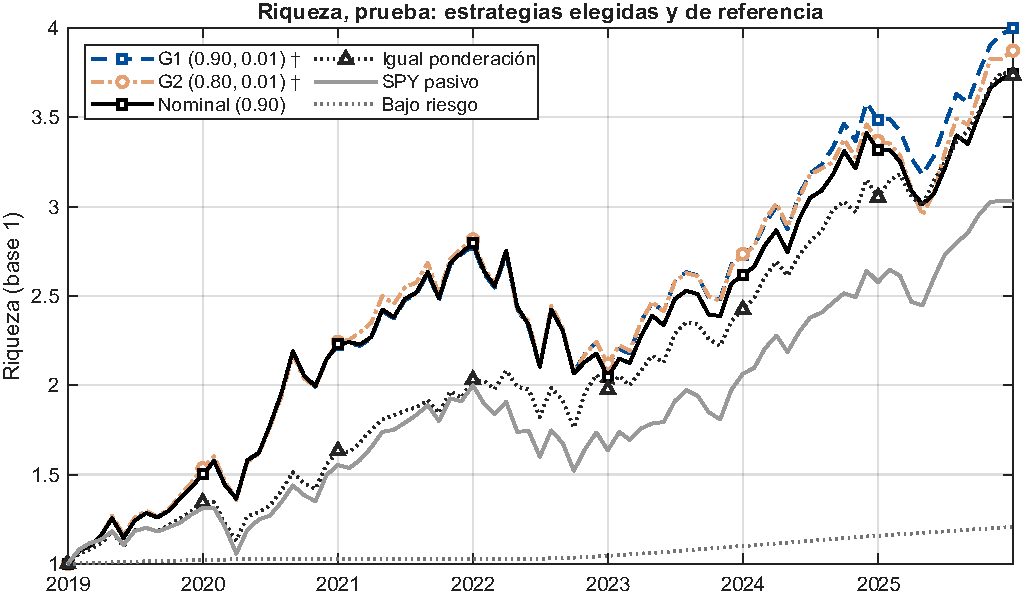
\includegraphics[width=\textwidth]{results_finales/figuras/riqueza_referencias_prueba.pdf}
\caption{Prueba 2019--2025: riqueza re-basada a 1 de las configuraciones elegidas, el nominal con $\delta=0.90$ y las estrategias de referencia.}\label{fig:riqueza_referencias}
\end{figure}

\begin{figure}[htbp]
\centering
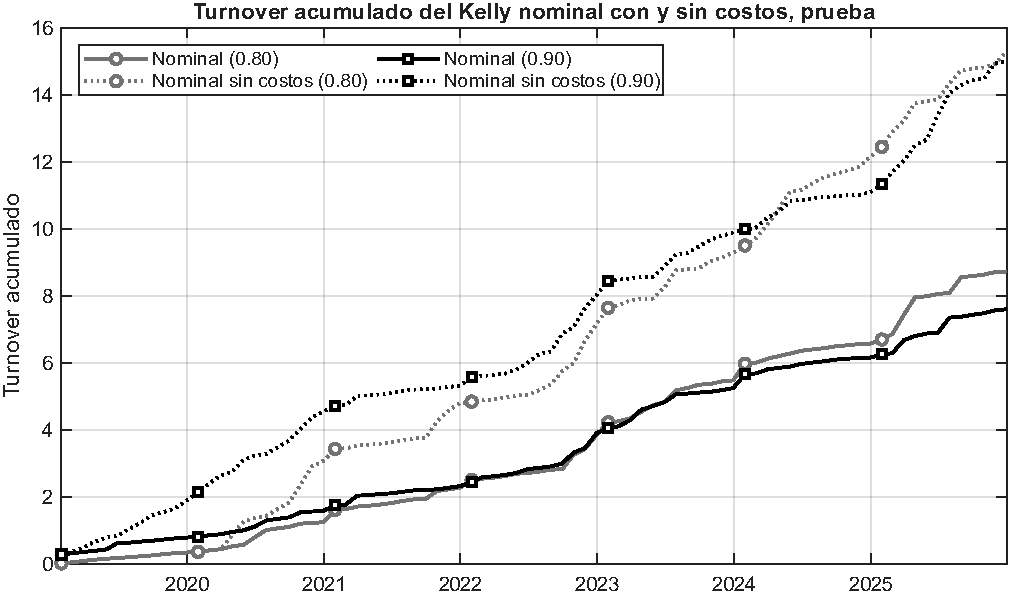
\includegraphics[width=0.85\textwidth]{results_finales/figuras/turnover_con_sin_costos_prueba.pdf}
\caption{Prueba 2019--2025: turnover acumulado del Kelly nominal con $\tau=0.001$ y con $\tau=0$, para $\delta=0.80$ y $0.90$.}\label{fig:turnover_costos}
\end{figure}

% ---------------------------------------------------------------------
\FloatBarrier %%% [R-res] las flotantes de la subsección anterior no pasan de aquí
\subsection{Distribución adversarial de cada geometría}\label{sec:res_adversarial}

%%% [fuente] complementarias/tabla_h_adversarial.csv y TABLAS_R8.md (r8_tiempos_adversarial.m).
%%% [R-res] Se reporta el caso "común" (mismo portafolio), que aísla la geometría. La explicación del patrón
%%% (G2 restringe al adversario a perturbaciones dentro del mismo estado de mercado) es una hipótesis: va a la Discusión.
Para ver cómo reponderan los escenarios las dos geometrías se calculó, en cada fecha de decisión, la distribución adversarial $p$ frente a un mismo portafolio, el Kelly nominal con el mismo $\delta$, de modo que solo cambia la geometría (Tabla~\ref{tab:adversarial}). Con $\eta=0.01$ la perturbación es pequeña: en prueba, el adversario movió en promedio entre $0.97\,\%$ y $1.33\,\%$ de la masa de probabilidad, el número efectivo de escenarios se mantuvo entre $58.8$ y $59.3$ de 60 y la masa del peor escenario estuvo entre $1.72\,\%$ y $1.93\,\%$, frente a $1/60\approx1.67\,\%$. El presupuesto de transporte $\rho_k$ se agotó en todas las fechas.

Las geometrías difieren en hacia dónde va esa masa. Con $c_1$, la geometría~1 asignó a los meses de la ventana con retorno de SPY negativo un exceso medio de $0.65$ puntos porcentuales sobre su frecuencia empírica, positivo en el $73.8\,\%$ de las fechas; la geometría~2, $0.39$ puntos, positivo en el $40.5\,\%$. Con $c_2$ las cifras son $0.89$ y $0.42$ puntos ($94.0\,\%$ y $50.0\,\%$ de las fechas). En los meses con VIX alto el exceso de la geometría~2 fue nulo o negativo con $c_1$ ($-0.02$ puntos, frente a $0.13$ de la geometría~1). La diferencia es mayor en validación: con el mismo portafolio, la geometría~1 trasladó masa extra a los meses con SPY negativo en el $89.6\,\%$ de las fechas y la geometría~2 en el $2.1\,\%$. La Figura~\ref{fig:exceso_spy} muestra que en prueba las dos geometrías se acercan en 2019--2020 y que desde 2023 hay tramos en los que coinciden o la geometría~2 supera a la geometría~1.

% Generado por results_finales/r8_tiempos_adversarial.m; no editar a mano.
\begin{table}[h]
\centering
\footnotesize
\setlength{\tabcolsep}{4pt}
\caption{Prueba 2019--2025: distribución adversarial $p$ de la bola de Wasserstein frente a un mismo portafolio (el Kelly nominal con el mismo $\delta$), de modo que solo cambia la geometría. Medias sobre las 84 fechas de decisión. Masa movida: $\frac12\sum_s|p_s-1/N|$. Exceso de masa: masa adversarial en los meses de la ventana con VIX sobre su mediana (o con retorno de SPY negativo) menos la fracción de esos meses. Fechas con exceso $>0$: con umbral $10^{-8}$. Descriptivo.}\label{tab:adversarial}
\begin{tabular}{|l|r|r|r|r|}
\hline
 & \multicolumn{2}{c|}{\textbf{$c_1=(0.90,\,0.01)$}} & \multicolumn{2}{c|}{\textbf{$c_2=(0.80,\,0.01)$}} \\ \cline{2-5}
\textbf{Indicador} & \textbf{G1} & \textbf{G2} & \textbf{G1} & \textbf{G2} \\ \hline
$\rho_k$ medio & 0.0083 & 0.0083 & 0.0083 & 0.0083 \\ \hline
Masa movida (\%) & 1.10 & 1.32 & 0.97 & 1.33 \\ \hline
Número efectivo de escenarios (de 60) & 59.1 & 58.8 & 59.3 & 58.8 \\ \hline
Masa del peor escenario (\%; $1/N=1.67$) & 1.81 & 1.72 & 1.93 & 1.83 \\ \hline
Exceso de masa, VIX alto (pp) & 0.13 & $-$0.02 & 0.13 & 0.09 \\ \hline
Fechas con exceso $>0$, VIX alto (\%) & 33.3 & 6.0 & 29.8 & 11.9 \\ \hline
Exceso de masa, $r^{\mathrm{SPY}}<0$ (pp) & 0.65 & 0.39 & 0.89 & 0.42 \\ \hline
Fechas con exceso $>0$, $r^{\mathrm{SPY}}<0$ (\%) & 73.8 & 40.5 & 94.0 & 50.0 \\ \hline
\end{tabular}
\end{table}


\begin{figure}[htbp]
\centering
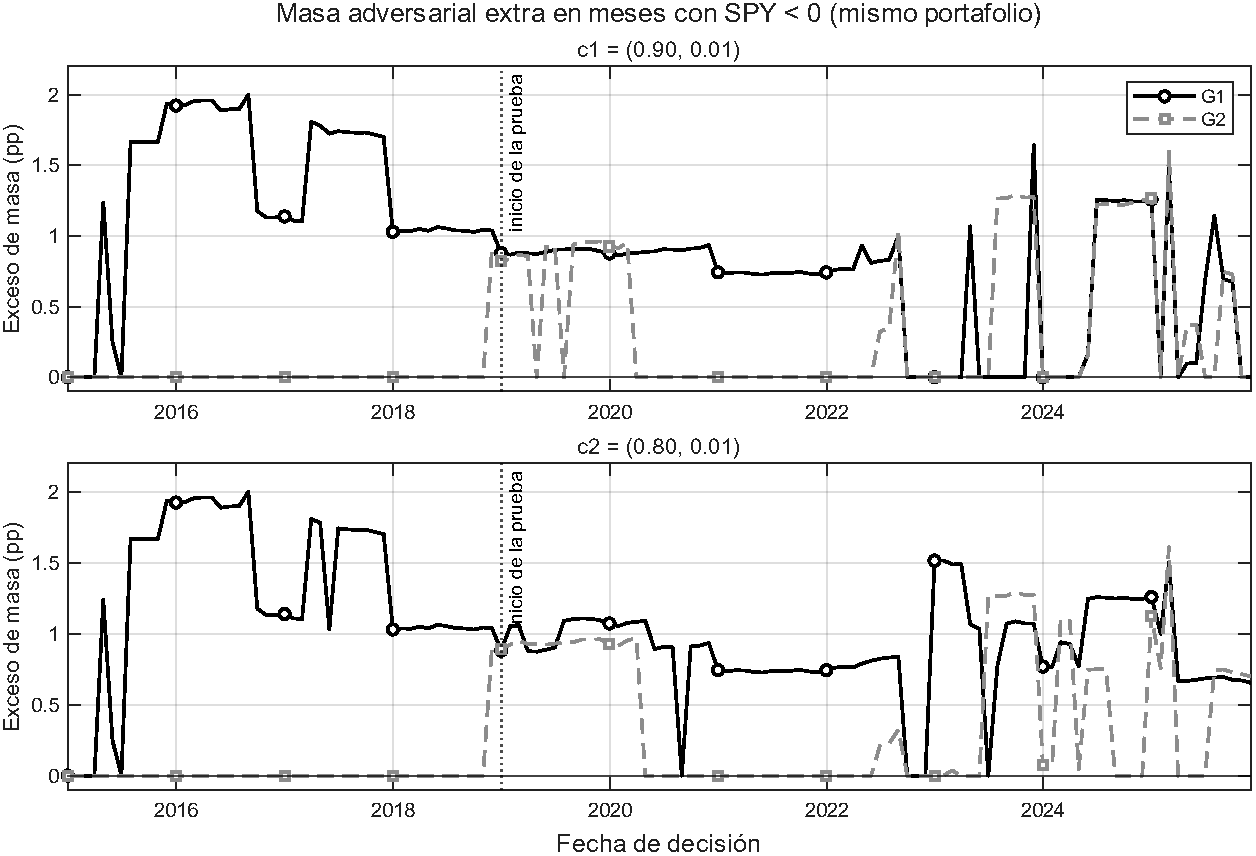
\includegraphics[width=\textwidth]{results_finales/complementarias/exceso_spy_negativo.pdf}
\caption{Exceso de masa adversarial (puntos porcentuales) en los meses de la ventana con retorno de SPY negativo, frente a un mismo portafolio, en las 132 fechas de decisión. La línea punteada marca la primera decisión del periodo de prueba.}\label{fig:exceso_spy}
\end{figure}

% ---------------------------------------------------------------------
\FloatBarrier %%% [R-res] las flotantes de la subsección anterior no pasan de aquí
\subsection{Síntesis}\label{sec:res_sintesis}

%%% [fuente] RESULTADOS.md §2 y §3.
En síntesis: (i) la implementación fue numéricamente estable y reprodujo el nominal con $\eta=0$; (ii) en validación todo $\eta>0$ redujo la riqueza, con $\eta\ge0.30$ ambas geometrías se fueron a bajo riesgo y la regla de selección eligió $\eta=0.01$ en las dos; (iii) en prueba, con parámetros emparejados, no se encontró una diferencia media de crecimiento entre la geometría informada por el mercado y la de solo retornos, y las diferencias en pérdidas, concentración y costos fueron pequeñas y sin un signo consistente entre valores de $\delta$; (iv) las estrategias robustas terminaron la prueba con más riqueza, menos turnover y menos costo que el nominal del mismo $\delta$, de forma descriptiva y con un único intervalo exploratorio que excluye el cero; y (v) con el mismo portafolio, la geometría~2 asignó menos masa adversarial adicional que la geometría~1 a los meses de retorno de mercado negativo. Los resultados no permiten ordenar las estrategias a partir de la riqueza final, afirmar diferencias entre regímenes ni generalizar fuera del universo y del periodo estudiados.

%%% [R-res] Ninguna flotante pasa de aquí (antes de la bibliografía).
\FloatBarrier
